%!TEX root = ../dokumentation.tex

\chapter{Dockerfile}
\label{ch:Dockerfile}
Das Dockerfile legt das Image für die später folgenden Anwendungscontainer fest. Der DockercomposeBereich "microservice-web" und der dortige build . Befehl referenziert auf dieses Dockerfile.

\begin{wrapfigure}{r}{0\textwidth}
\centering
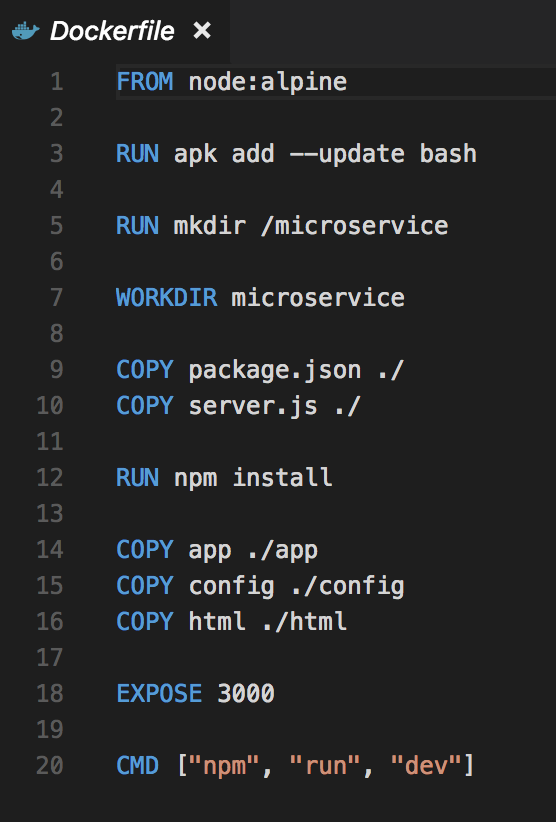
\includegraphics[height=.6\textwidth]{Dockerfile.png}
\vspace{3pt}
\caption{Schaubild\footnotemark}
\label{fig:blueant}
\end{wrapfigure}

Zeile 1: FROM node:alpine legt das Betriebssystem des Containers fest. Hier wird auf eine Alpine-Maschine mit vorinstalliertem Node.js zurückgegriffen. Dieses System ist sehr beliebt für einfache Anwendungen und wird häufig für kleine Projekte verwendet, da es sehr geradlinig aufgebaut ist und wenig Ressourcen benötigt.

Zeile 3: RUN beschreibt eine Eingabe in die virtuelle Kommandozeile. apk add --update bash installiert die aktuelle Version von bash auf dem containerisierten Betriebssystem.

Zeile 5 bis Zeile 10: Die folgenden Kommandos erstellen einen Ordner auf dem Container, ändern das Arbeitsdirectory auf den neu erstellten Ordner und kopiert die Dateien package.json und server.js von der Festplatte des Aufrufers in den neu erstellten Ordner des Containers.

Zeile 12: npm install führt die Installation der Dependencies aus der kopierten package.json aus.

Zeile 14 bis Zeile 16: Die hier folgenden COPY-Befehle kopieren die Ordner app, config und html vom Host auf den Container.

Zeile 18: EXPOSE beschreibt den Port auf den der Container später hört.

Zeile 20: Das Kommando CMD beschreibt die final-ausgeführten Befehle. In diesem Fall "npm run dev" welches in der package.json festgelegt wurde und die Anwendung im Developmentmodus startet. An dieser Stelle könnte auch ein Releasekommando eingeführt werden)